\documentclass[portuguese]{sbc2025}%

%\usepackage{graphicx}% já está incluido na classe
%\usepackage[utf8]{inputenc} % obsoleto, desnecessário

\usepackage[misc,geometry]{ifsym}

%%%%  %\usepackage{fontspec}

%% Os problemas com a classe eram originados por carregarem ambos os
%% pacotes fontenc e fontspec simultaneamente. Agora a classe detecta
%% qual engine está em uso e se for o pdflates então carrega o
%% fontenc. Se forem o xelatex ou lualatex então carrega o
%% fontspec. Eu particularemnte prefiro o lualatex ou o xetex


% \usepackage{fontawesome} %%% incluido na classe. Desnecessário
% chamá-lo aqui


%%%% \usepackage{academicons}
%%%% outro encrenqueiro que se tornou desnecessario. Deste typeface só
%%%% se usava o glifo do orcid e o codigo interno bombava.
%%%% Substitui pelo pacote orcidlink (carregado internamete na classe)
%%%% e consertei o codigo na classe.


%\usepackage{color} % carregada dentro da classe
%\usepackage{hyperref} % carregada dentro da classe

\usepackage{aas_macros}
\usepackage[bottom]{footmisc}

%\usepackage{supertabular}
%\usepackage{multicol}
%\usepackage{multirow}
%% O pacote tabularray é muito melhor para
% a criacao de tabela complexas e/ou loooongas; tudo de modo simples.
%% Torna o uso de multicol e multirow desnecessarios

% \usepackage{tabularray} % não utilizado nesta versão.


\usepackage{afterpage}
\usepackage{url}
\usepackage{pifont}


\setcitestyle{square}


\definecolor{engtitle}{rgb}{0.5,0.5,0.5}
\definecolor{orcidlogo}{rgb}{0.37,0.48,0.13}
\definecolor{unilogo}{rgb}{0.16, 0.26, 0.58}
\definecolor{maillogo}{rgb}{0.58, 0.16, 0.26}
\definecolor{darkblue}{rgb}{0.0,0.0,0.0}
\hypersetup{colorlinks,breaklinks,
            linkcolor=darkblue,urlcolor=darkblue,
            anchorcolor=darkblue,citecolor=darkblue}
%\hypersetup{colorlinks,citecolor=blue,linkcolor=blue,urlcolor=blue}

%%%%%%% IMPORTANT: We disable hyperlinks by default with this line, to avoid the error "\pdfendlink ended up in different nesting level" while writing.
%\hypersetup{draft}

\jid{ENIAC}
\jtitle{Anais do Encontro Nacional de Inteligência Artificial e Computacional, 202X, XX:1}
\issn{XXXX-XXXX}
\doi{10.5753/eniac.202X.XXXXXX}
\copyrightstatement{This work is licensed under a Creative Commons Attribution 4.0 International License}
\jyear{202X}

\category{Artigo de Pesquisa/Research Paper}
\title[Diagnóstico Personalizado de Carteiras com LLMs Multiagente]{Diagnóstico Personalizado de Carteiras Financeiras com Sistemas Multiagente baseados em LLMs}
\engtitle{\textcolor{engtitle}{Personalized Financial Portfolio Diagnosis with LLM-based Multi-Agent Systems}}

%THE ORCID IS MANDATORY FOR EACH AUTHOR IN JBCS
\author[Florenzano et al. 202X]{
\affil{\textbf{Rafael Marins Florenzano}~\orcidlink{0009-0003-0347-7795}~\textcolor{blue}{\faEnvelopeO}~~[{Universidade de Fortaleza (UNIFOR)}~|\href{mailto:rafaelmarins2003@gmail.com}{~{\textit{rafaelmarins2003@gmail.com}}}~]}

\affil{\textbf{Rian Maia de Freitas}~\orcidlink{0009-0005-4083-7432}~~[{Universidade de Fortaleza (UNIFOR)}~|\href{mailto:rianmaiaf@gmail.com}{{\textit{rianmaiaf@gmail.com}}}~]}

}

\begin{document}

\begin{frontmatter}

\maketitle

\begin{mail}
Universidade de Fortaleza (UNIFOR), Av. Washington Soares, 1321, Edson Queiroz, Fortaleza, CE, 60811-905, Brasil.
\end{mail}


\begin{abstract-pt}
Sistemas multiagente baseados em modelos de linguagem têm sido propostos
para análise financeira, mas seus ganhos sobre baselines fortes de agente
único permanecem incertos. Este artigo propõe uma arquitetura multiagente
para diagnóstico personalizado de carteiras financeiras, combinando agentes
especialistas (técnico, fundamentalista, sentimento, macroeconômico e de
risco), debate adversarial Bull/Bear com moderação, roteamento heterogêneo
de modelos por papel e saídas estruturadas. A avaliação compara a arquitetura
contra quatro baselines, incluindo agente único com self-consistency e
multiagente sem debate. O estudo inclui uma validação estrutural em 43
carteiras brasileiras e uma comparação principal entre técnicas em 20
carteiras enriquecidas com dados de mercado. No cenário enriquecido, o
baseline multiagente sem debate apresenta o melhor equilíbrio entre
concordância com consenso, diagnósticos conclusivos e custo proxy. O
roteamento heterogêneo reduz custo e latência em relação ao debate
homogêneo, mas ainda não demonstra ganho claro de acurácia proxy.
\end{abstract-pt}

\begin{abstract-en}
Large language model based multi-agent systems have been proposed for
financial analysis, but their gains over strong single-agent baselines
remain unclear. This paper proposes a multi-agent architecture for
personalized portfolio diagnosis, combining specialist agents (technical,
fundamental, sentiment, macroeconomic and risk), an adversarial bull/bear
debate with moderation, heterogeneous model routing per role, and
structured outputs. The architecture is compared against four baselines,
including a single-agent with self-consistency and a multi-agent setup
without debate. The study includes a structural validation over 43 Brazilian
stock portfolios and a main comparison among techniques over 20 portfolios
enriched with market data. In the enriched setting, the multi-agent baseline
without debate provides the best balance between consensus agreement,
conclusive diagnoses and cost proxy. Heterogeneous routing reduces cost and
latency compared with the homogeneous debate variant, but does not yet show a
clear proxy-accuracy gain.
\end{abstract-en}

\begin{pchaves}
LLMs, sistemas multiagente, diagnóstico financeiro, carteiras, avaliação experimental
\end{pchaves}

\begin{keywords}
LLMs, multi-agent systems, financial diagnosis, portfolios, experimental evaluation
\end{keywords}

\begin{dates}
% This information will be provided by the editor before publishing the paper
\noindent{\sffamily\textbf{Recebido/Received:}} DD Month YYYY~~~$\bullet$~~~
{\sffamily\textbf{Aceito/Accepted:}} DD Month YYYY~~~$\bullet$~~~
{\sffamily\textbf{Publicado/Published:}} DD Month YYYY
\end{dates}


%\begin{license}
%Published under the Creative Commons Attribution 4.0 International Public License (CC BY 4.0)
%\end{license}

\end{frontmatter}


\section{Introdução}
\label{sec:intro}

Modelos de linguagem de grande escala (LLMs) vêm sendo incorporados a sistemas
multiagente para apoiar análise financeira: interpretação de notícias, leitura
de indicadores, construção de teses de investimento e tomada de decisão em
ambientes de trading. O volume de propostas cresce, mas uma lacuna
metodológica permanece. Grande parte dos trabalhos atribui ganhos à presença
de múltiplos agentes ou ao uso de debate sem comparar os resultados contra
baselines fortes de agente único submetidos ao mesmo orçamento de
computação. Fica difícil, então, distinguir o que vem da arquitetura
multiagente do que vem, simplesmente, de um modelo mais capaz acompanhado
de prompts mais bem feitos.

A questão pesa especialmente no contexto financeiro. Uma resposta que soa
convincente pode não significar maior personalização ao investidor, melhor
cobertura dos fatores de risco da carteira ou menor taxa de erro factual
sobre os ativos analisados. Soma-se a isso o fato de que a maior parte dos
sistemas existentes prioriza recomendação de ativos ou decisão de compra e
venda, deixando em segundo plano um problema mais frequente na prática:
diagnosticar uma carteira já constituída em relação ao perfil de risco, ao
horizonte e ao objetivo do usuário. Diagnosticar não é o mesmo que
recomendar. O objetivo deixa de ser propor movimentações sobre os ativos e
passa a ser explicar o estado atual da carteira, apontar fatores de
atenção e sinalizar quando a evidência disponível é insuficiente.

Este trabalho propõe uma arquitetura multiagente baseada em LLMs para
diagnóstico personalizado de carteiras financeiras. A saída do sistema é
uma classificação discreta da carteira frente ao perfil informado, com
justificativa textual, fatores positivos, fatores negativos e nível de
confiança. Não há recomendações de compra, venda ou rebalanceamento, e o
sistema não assume papel de aconselhamento financeiro. Para sustentar
afirmações sobre o impacto da arquitetura, a proposta é avaliada contra um
conjunto de baselines que inclui agente único ingênuo, agente único com
raciocínio estruturado e self-consistency, e multiagente sem debate, sob
mesma entrada e mesmo formato de saída.

As principais contribuições deste trabalho são:

\begin{itemize}
  \item uma arquitetura multiagente para diagnóstico personalizado de
  carteiras, organizada em agentes especialistas (técnico, fundamentalista,
  sentimento, macroeconômico e de risco), um par adversarial Bull/Bear e um
  moderador que produz a classificação final;
  \item um mecanismo de debate adversarial Bull/Bear com síntese por
  moderador e suporte a roteamento heterogêneo de modelos por papel, que
  permite isolar o efeito da arquitetura do efeito do modelo subjacente;
  \item uma metodologia de avaliação que compara o sistema proposto contra
  baselines fortes de agente único, self-consistency e multiagente sem
  debate, usando entrada congelada e saída estruturada para garantir
  comparações controladas;
  \item um pipeline de rastreabilidade que registra, por execução, chamadas
  realizadas, latência, tokens, erros de parsing e respostas estruturadas,
  permitindo reproduzir e auditar tanto a arquitetura proposta quanto os
  baselines.
\end{itemize}

\section{Trabalhos Relacionados}

\subsection{Sistemas multiagente com LLMs em finanças}

Trabalhos recentes vêm explorando agentes baseados em LLMs para análise
financeira e para tomada de decisão em trading. TradingAgents organiza
diferentes papéis (analistas de notícias, analistas técnicos, gerentes de
risco e traders) em fluxos de comunicação que terminam em decisões
operacionais \citep{tradingagents2024}. FinCon propõe um sistema com
reforço verbal conceitual para apoiar decisões financeiras complexas,
explorando como agentes podem revisar suas próprias conclusões a partir de
sinais contextuais \citep{fincon2024}. AlphaAgents foca especificamente em
construção de carteiras de ações usando múltiplos agentes baseados em LLMs
\citep{alphaagents2025}, e HedgeAgents discute uma abordagem multiagente
voltada ao suporte à decisão em fundos \citep{hedgeagents2025}. Em comum,
essas propostas decompõem a tarefa em papéis especializados e combinam os
resultados desses papéis em uma decisão final.

O foco predominante, contudo, está em seleção de ativos ou em decisão de
compra e venda. O presente trabalho se posiciona em outro recorte: tratar o
problema como diagnóstico personalizado de uma carteira já existente,
condicionado ao perfil declarado pelo usuário. A unidade de avaliação
deixa de ser apenas a plausibilidade de uma tese de investimento e passa
a incluir a adequação da classificação aos diferentes perfis e a
capacidade do sistema de indicar incerteza quando faltam dados. Isso
afeta diretamente as métricas escolhidas: além de variáveis operacionais,
importam sensibilidade à personalização e cobertura dos fatores de risco.

\subsection{Debate multiagente e baselines fortes}

Debate entre múltiplos agentes baseados em LLMs tem sido proposto como
estratégia para melhorar raciocínio, robustez e verificação cruzada de
respostas. Evidências recentes, porém, mostram que parte dos ganhos
atribuídos ao debate desaparece quando se utilizam baselines de agente
único com orçamento computacional equivalente, com prompts melhores e
self-consistency \citep{zhang2025stop}. O ponto é especialmente relevante
em domínios com alto custo cognitivo, como o financeiro, onde acrescentar
chamadas a uma LLM se traduz em mais latência e mais custo por análise.

Por isso, este trabalho adota baselines fortes de agente único como
referência principal de comparação. Em particular, considera-se uma LLM
única com raciocínio estruturado e self-consistency, com orçamento
ajustado ao número de chamadas dos demais baselines, de modo a evitar que
diferenças observadas decorram apenas da maior alocação de computação em
sistemas multiagente. O sistema sem debate, com agentes especialistas e
moderador, entra como ponto intermediário e permite separar o efeito do
debate do efeito da decomposição em papéis.

\subsection{Personalização em diagnóstico financeiro}

Personalização aparece frequentemente como característica desejável em
aplicações financeiras com LLMs, mas raramente como dimensão de avaliação
em si. Em muitos sistemas, o perfil do usuário é passado como entrada sem
que se verifique, de forma controlada, se a saída de fato muda com esse
perfil. O risco é claro: respostas pouco condicionadas ao usuário, em que
o sistema repete diagnósticos genéricos sobre a carteira independente do
perfil declarado.

Aqui, a personalização é avaliada por meio de casos contrafactuais. A
mesma carteira é diagnosticada sob perfis conservador, moderado e
agressivo, com todas as demais entradas constantes. A expectativa é que a
classificação e a justificativa se desloquem na direção compatível com
cada perfil: uma carteira de alta volatilidade deve ser mais
frequentemente classificada como \textit{atenção} ou \textit{risco
elevado} sob perfil conservador do que sob perfil agressivo. A frequência
com que essa relação se sustenta passa a ser, então, uma métrica direta
de sensibilidade à personalização, e separa comportamento personalizado
de mera variação textual.

\section{Arquitetura Proposta}

Esta seção descreve a arquitetura proposta para diagnóstico personalizado de
carteiras. O sistema recebe uma entrada estruturada, executa agentes
especialistas com papéis financeiros distintos, promove um debate
adversarial entre interpretações contrastantes e produz uma saída final
padronizada. A arquitetura não tem por objetivo recomendar compra, venda
ou rebalanceamento: sua função é classificar a situação da carteira em
relação ao perfil do usuário e tornar explícitos os fatores que sustentam
essa classificação. O recorte por diagnóstico, em vez de recomendação, é
deliberado. Ele permite que o sistema admita incerteza, separe risco
observado de lacuna de dados e seja avaliado por métricas que não dependem
de execução em mercado real.

\subsection{Entrada, estado compartilhado e saída}

A entrada do sistema é composta por três grupos de informação. O primeiro
é a carteira, representada por tickers, pesos normalizados e setores. O
segundo é o perfil do usuário, contendo tolerância a risco, horizonte e
objetivo declarado. O terceiro contém dados financeiros externos, quando
disponíveis: preços, fundamentos, notícias e indicadores macroeconômicos.
A separação é intencional. A arquitetura segue operacional mesmo quando
parte dos dados externos não está presente, registrando as lacunas em vez
de inferir o que não foi observado.

Internamente, a execução mantém um estado compartilhado que armazena a
entrada original, as análises produzidas pelos especialistas, as rodadas
de debate, o diagnóstico final e metadados de execução. Cada agente lê o
estado e retorna apenas uma atualização parcial, sem sobrescrever
resultados de outros papéis. A organização também facilita a comparação
com os baselines: o mesmo estado inicial pode ser consumido por uma LLM
única, por um conjunto de especialistas sem debate ou pela arquitetura
completa, mantendo a entrada controlada entre as variantes.

A saída final é um objeto estruturado com cinco campos principais:
classificação discreta, justificativa textual, fatores positivos, fatores
negativos e confiança. As classes possíveis são \textit{estável},
\textit{atenção}, \textit{risco elevado}, \textit{desalinhada} e
\textit{inconclusiva}. A classe \textit{inconclusiva} é central no
problema: ela dá ao sistema um caminho explícito para sinalizar falta de
evidência, em lugar de produzir uma análise aparentemente segura sem base
informacional. Respostas inconclusivas justificadas por ausência de dados
são tratadas, nas métricas, de forma distinta das classificações
afirmativas, para não penalizar o sistema por reconhecer suas próprias
limitações.

\subsection{Agentes especialistas}

Os agentes especialistas decompõem o diagnóstico em perspectivas
financeiras complementares. O agente técnico resume sinais de preço,
médias móveis, volatilidade e tendência, quando esses dados estão
disponíveis. O agente de sentimento interpreta notícias, eventos e
evidências textuais explicitamente fornecidas. O agente fundamentalista
avalia indicadores como valuation, dividendos, margens, lucro e dívida.
O agente macroeconômico resume fatores agregados relevantes para a
carteira, como ciclo de juros e condições setoriais amplas. O agente de
risco avalia concentração, exposição setorial e alinhamento da carteira
ao perfil informado.

A decomposição não assume que cada agente terá evidência suficiente. Uma
regra central dos prompts é distinguir risco observado de lacuna de
dados. Ausência de fundamentos, por exemplo, não deve ser tratada como
fundamento ruim; ela deve ser registrada como incerteza explícita. A
distinção é importante sobretudo na comparação com baselines de agente
único, que tendem a produzir respostas mais assertivas mesmo sob baixa
evidência, escondendo a fragilidade do diagnóstico em texto bem
formulado.

Todos os agentes retornam saídas estruturadas via schemas Pydantic. O
sistema envia o schema esperado no prompt e valida a resposta localmente.
Respostas que não obedecem ao schema são registradas como erro de parsing
e não compõem o diagnóstico final, evitando que saídas malformadas
contaminem as métricas. A taxa de sucesso de parsing é tratada como
métrica operacional explícita e reportada para todos os baselines, como
indicador da confiabilidade do sistema em uso contínuo.

\subsection{Debate adversarial}

O debate adversarial é composto por dois agentes contrastantes. O agente
Bull constrói a leitura favorável mais forte compatível com os dados
disponíveis; o agente Bear, a leitura crítica mais forte. Ambos são
instruídos a não recomendar compra, venda ou rebalanceamento e a não
transformar lacunas de dados em perdas financeiras. O moderador recebe as
duas leituras junto com as análises dos especialistas e produz a síntese
final, atribuindo à classificação um nível de confiança coerente com o
grau de convergência entre as fontes.

O objetivo do debate não é decidir por votação, e sim explicitar
incertezas e fatores contrastantes. Cabe ao Bull organizar evidências
favoráveis e mitigadores; cabe ao Bear tornar visíveis riscos,
fragilidades e pressupostos pouco sustentados. Trata-se, na prática, de
um mecanismo de auditoria interna. Quando Bull e Bear convergem, a
confiança do diagnóstico cresce. Quando divergem fortemente, há razão
para uma classificação intermediária, como \textit{atenção}, ou para uma
classificação \textit{inconclusiva}.

O debate é limitado por um número máximo de rodadas e por uma medida
determinística de convergência lexical entre rodadas, calculada sobre a
interseção dos fatores mencionados por Bull e Bear. A configuração
avaliada utiliza uma rodada por caso, o que mantém a comparação com os
baselines transparente: o custo adicional do debate fica diretamente
refletido no número de chamadas LLM, em tokens e em latência, todos
registrados por execução.

\subsection{Roteamento de modelos}

São avaliadas duas variantes da arquitetura com debate. A variante B4-H
emprega um único modelo em todos os papéis, isolando o efeito da
arquitetura em relação ao modelo subjacente. A variante B4-R utiliza
roteamento heterogêneo, combinando modelos distintos para especialistas,
debate e moderação. O limite de concorrência é configurável e foi ajustado
conforme a estabilidade do provedor. A validação estrutural usou até três
chamadas simultâneas; parte da comparação enriquecida foi reduzida para uma
chamada por vez após respostas temporárias de sobrecarga do serviço. Essa
diferença é registrada nos logs e entra nas métricas operacionais de
latência e chamadas, sem alterar a entrada compartilhada entre baselines.

Na configuração avaliada, B4-H utiliza \texttt{deepseek-v4-pro} em todos
os papéis. Em B4-R, os agentes técnico e de risco utilizam
\texttt{nemotron-3-super}; sentimento, fundamentos, macroeconomia e
moderação utilizam \texttt{deepseek-v4-pro}; Bull e Bear utilizam
\texttt{minimax-m2.7}. As páginas oficiais do Ollama classificam
\texttt{deepseek-v4-pro} como uso ``extra high'', e
\texttt{minimax-m2.7} e \texttt{nemotron-3-super} como uso ``medium''
\citep{ollamadeepseek2026,ollamaminimax2026,ollamanemotron2026}. A escolha
de modelos por papel não é apresentada como ótima em sentido absoluto. Ela
operacionaliza a hipótese de que papéis diferentes podem se beneficiar de
modelos com perfis distintos, enquanto B4-H atua como controle homogêneo
dessa hipótese.

\subsection{Implementação e rastreabilidade}

A arquitetura é implementada em Python, com LangGraph para orquestração
do estado compartilhado entre agentes e Pydantic para os schemas de
entrada e saída. As chamadas aos modelos passam por uma camada uniforme,
o que permite trocar provedores sem alterar a lógica dos agentes. Cada
chamada LLM passa por um envelope que registra o agente de origem, o
baseline em execução, o caso analisado, o modelo utilizado e o tempo de
resposta.

A execução completa registra, em SQLite, informações detalhadas por
caso, baseline, agente e chamada LLM: modelo, prompt enviado, resposta
bruta, resposta parseada, status, latência, tokens quando disponíveis e
erro quando aplicável. Os registros sustentam tanto a depuração quanto
as métricas reportadas, e permitem reexecutar análises agregadas sem
acionar novamente os modelos. Em outras palavras, é possível auditar de
forma objetiva se diferenças entre baselines vêm de mudanças na
arquitetura, do modelo utilizado ou de comportamento intermitente do
provedor.

\section{Metodologia Experimental}

\subsection{Workload}

O workload contém 43 carteiras de ações brasileiras obtidas de fontes
públicas e organizadas em formato estruturado. Cada carteira possui pesos
normalizados, setores e metadados de origem. O conjunto reúne 88 tickers
únicos e cobre três perfis de investidor: conservador, moderado e
agressivo. As carteiras são consumidas pela arquitetura e pelos baselines
exatamente na mesma forma estruturada, sem alterações específicas por
abordagem.

O estudo usa duas execuções com funções diferentes. A primeira é uma
validação estrutural sobre as 43 carteiras usando apenas carteira e perfil.
Ela verifica se todas as variantes executam de forma comparável e como cada
uma trata lacunas de informação, mas não é usada como principal evidência de
qualidade financeira. A segunda é a comparação principal entre técnicas:
um subconjunto de 20 carteiras é enriquecido com preços via
\texttt{yfinance}, notícias e sinais textuais via Brave Search API, e
indicadores macroeconômicos via fontes públicas. Essa execução enriquecida
é o cenário usado para comparar custo, detalhamento, conclusividade e proxy
de acurácia entre B1, B2, B3, B4-H e B4-R.

\subsection{Baselines}

A avaliação compara cinco variantes:

\begin{itemize}
  \item B1: LLM única ingênua, com prompt direto;
  \item B2: LLM única com raciocínio estruturado e self-consistency;
  \item B3: sistema multiagente com especialistas e moderador, sem debate;
  \item B4-H: sistema multiagente com debate usando um modelo homogêneo;
  \item B4-R: sistema multiagente com debate e roteamento heterogêneo por
  papel.
\end{itemize}

Todos os baselines recebem a mesma entrada congelada e produzem o mesmo
formato de saída: classificação, justificativa, fatores positivos,
fatores negativos, confiança e alinhamento ao perfil. A uniformidade é
indispensável para comparações justas e permite que as métricas
reportadas sejam computadas exatamente da mesma forma para todos os
baselines. B1, B2 e B3 atuam como pontos de referência de exigência
crescente, de modo que B4-H e B4-R precisam superar não apenas o
baseline ingênuo, mas também variantes deliberadamente fortes de agente
único e de multiagente sem debate.

\subsection{Métricas}

As métricas estão organizadas em três grupos. As operacionais incluem
taxa de sucesso final, latência fim a fim, número de chamadas LLM,
tentativas com erro transitório ou de parsing, tokens por baseline e
custo por análise. Como o provedor usado nos experimentos, Ollama Cloud,
mede uso por utilização de infraestrutura e não por tarifa pública fixa
por token, o custo é reportado de duas formas. A primeira é um proxy de
uso no Ollama, calculado como tokens multiplicados pelo nível oficial de
uso do modelo. A segunda é uma estimativa contrafactual em dólares usando
preços oficiais por token quando eles estão disponíveis para o provedor
original do modelo. Para DeepSeek V4-Pro e MiniMax M2.7 há preço público
por token; para Nemotron 3 Super, usado via Ollama Cloud, não foi
encontrada uma tarifa oficial equivalente por token, então seus tokens
são reportados separadamente como não precificados
\citep{deepseekpricing2026,minimaxpricing2026,ollamapricing2026}.

As métricas estruturadas incluem a distribuição de classificações,
a taxa de diagnósticos conclusivos e uma medida de concordância com
consenso. Essa concordância é usada como proxy de acurácia: para cada
carteira, calcula-se a classe majoritária entre os cinco baselines e
mede-se se cada baseline concordou com essa maioria. Casos empatados são
excluídos do denominador. Essa métrica não mede acerto financeiro real;
ela mede consistência relativa entre modos de execução sob a mesma
entrada. As métricas textuais incluem quantidade média de fatores
positivos e negativos e tamanho médio da justificativa.

Nesta etapa do estudo, ainda não há ground truth humano nem comparação
com retorno futuro das carteiras. Por isso, a sensibilidade à
personalização, a consistência entre execuções e a avaliação textual com
anotação humana permanecem como próximos passos experimentais. Essa
separação evita tratar fluidez textual ou assertividade aparente como
prova de superioridade financeira.

\subsection{Rastreabilidade}

Cada execução registra em SQLite o baseline, o caso, o agente, o modelo,
o prompt, a resposta bruta, a resposta parseada, o status, a latência,
os tokens consumidos e o erro quando aplicável. A rastreabilidade tem
dois papéis. Primeiro, permite auditoria posterior e consolidação
quantitativa dos resultados sem novas chamadas LLM. Segundo, permite
distinguir comportamentos do sistema de comportamentos do provedor: se
um baseline apresentar variação anômala entre execuções, é possível
inspecionar diretamente os registros de chamadas e verificar se a
variação decorre de erros de parsing, de respostas atípicas do modelo
ou de mudanças sistemáticas no comportamento da arquitetura.

\section{Resultados}
\label{sec:resultados}

Os resultados foram obtidos em duas execuções com papéis distintos. A
primeira é uma validação estrutural: utiliza as 43 carteiras do workload
apenas com carteira e perfil, sem dados externos. Ela serve para confirmar
reprodutibilidade, tratamento de lacunas e custo operacional das variantes. A
segunda é a comparação principal entre técnicas no escopo financeiro: usa
20 carteiras com enriquecimento externo por preços, fundamentos, notícias
e indicadores macroeconômicos quando disponíveis. As conclusões sobre qual
modo teve melhor desempenho, qual foi mais detalhado e qual foi mais barato são
tiradas dessa execução enriquecida, sempre comparando baselines sob a mesma
entrada.

\subsection{Validação estrutural sem enriquecimento externo}

Essa validação processou 43 carteiras em cinco baselines, totalizando
215 diagnósticos. Todos os baselines finalizaram com status \texttt{ok}, sem
falha final de execução. A Tabela~\ref{tab:classificacoes-estrutural} mostra a
distribuição das classificações produzidas por cada abordagem.

\begin{table*}[!t]
\centering
\caption{Distribuição de classificações na validação estrutural com 43 carteiras.}
\label{tab:classificacoes-estrutural}
\begin{tabular}{@{}lrrrrr@{}}
\hline\hline
Baseline & Estável & Atenção & Risco elevado & Desalinhada & Inconclusiva \\
\hline
B1   & 12 & 8 & 0 & 0 & 23 \\
B2   & 11 & 8 & 1 & 0 & 23 \\
B3   &  0 & 0 & 0 & 1 & 42 \\
B4-H &  0 & 0 & 0 & 0 & 43 \\
B4-R &  0 & 0 & 0 & 2 & 41 \\
\hline\hline
\end{tabular}
\end{table*}

O resultado mais visível é que os baselines multiagente foram mais
conservadores na ausência de dados externos. B3, B4-H e B4-R
classificaram a maioria dos casos como \textit{inconclusiva}, enquanto
B1 e B2 produziram mais classificações afirmativas. Essa assimetria não
deve ser lida automaticamente como vantagem de B1 ou B2: os prompts
proíbem inventar dados ausentes, e uma classificação inconclusiva pode
ser a resposta correta quando a entrada contém apenas tickers, pesos,
setores e perfil do usuário.

A observação importa para o objetivo do artigo. O sistema proposto não
foi desenhado para sempre emitir uma opinião forte. Ele foi desenhado
para separar diagnóstico suportado por evidência de incerteza
informacional. A alta taxa de inconclusivos nos modelos multiagente
indica, então, que a decomposição em papéis e a moderação final
expõem mais as lacunas de dados do que os baselines de agente único.

\begin{table*}[!t]
\centering
\caption{Métricas operacionais na validação estrutural com 43 carteiras. P50 e P95 são percentis de latência fim a fim.}
\label{tab:operacional-estrutural}
\begin{tabular}{@{}lrrrrrrr@{}}
\hline\hline
Baseline & OK & Chamadas & Erros & Média (s) & P50 (s) & P95 (s) & Tokens/caso \\
\hline
B1   & 43 &  43 & 0 &  16.6 &   7.1 &  68.6 &  1\,162 \\
B2   & 43 & 215 & 0 &  31.5 &  16.0 & 106.2 &  6\,147 \\
B3   & 43 & 217 & 2 &  43.1 &  34.4 & 108.2 &  9\,525 \\
B4-H & 43 & 303 & 2 &  96.3 &  68.2 & 287.6 & 21\,879 \\
B4-R & 43 & 302 & 1 & 129.7 & 113.2 & 252.6 & 21\,467 \\
\hline\hline
\end{tabular}
\end{table*}

A Tabela~\ref{tab:operacional-estrutural} mostra o custo operacional de
cada variante. B1 é o mais barato, como esperado: realiza uma única
chamada por caso. B2 sobe o custo ao usar cinco amostras de
self-consistency. B3 tem custo próximo de B2 em número de chamadas,
mas distribui o trabalho entre agentes especializados. B4-H e B4-R são
as variantes mais caras, já que incluem especialistas, debate Bull/Bear
e moderação final. O acréscimo de custo é uma limitação prática da
arquitetura e precisa ser compensado por ganhos em qualidade
estruturada, auditabilidade ou controle de incerteza.

\subsection{Comparação principal com dados externos}

Para comparar os modos em um cenário financeiro mais realista, um
subconjunto de 20 carteiras foi executado com dados coletados
automaticamente: preços e fundamentos via \texttt{yfinance}, notícias via
Brave Search API e indicadores macroeconômicos de fontes públicas quando
disponíveis. Houve uma falha pontual de B4-H em um caso da primeira rodada
enriquecida, que foi reexecutado com sucesso. A análise abaixo usa os 100
resultados finais válidos e mantém a mesma entrada para todos os baselines.

\begin{table*}[!t]
\centering
\caption{Distribuição de classificações no subconjunto enriquecido com 20 carteiras.}
\label{tab:classificacoes-enriquecido}
\begin{tabular}{@{}lrrrrr@{}}
\hline\hline
Baseline & Estável & Atenção & Risco elevado & Desalinhada & Inconclusiva \\
\hline
B1   & 3 & 17 & 0 & 0 & 0 \\
B2   & 1 & 18 & 1 & 0 & 0 \\
B3   & 0 & 14 & 6 & 0 & 0 \\
B4-H & 0 &  9 & 5 & 1 & 5 \\
B4-R & 0 &  6 & 6 & 0 & 8 \\
\hline\hline
\end{tabular}
\end{table*}

Nesse cenário, B1, B2 e B3 produzem diagnósticos conclusivos em todos os
casos. B3, B4-H e B4-R também emitem mais classificações de
\textit{risco elevado}, o que é relevante para o escopo financeiro, pois
indica maior sensibilidade a fatores negativos da carteira. B4-H e B4-R
continuam mais cautelosos que os baselines de agente único, preservando uma
fração de diagnósticos inconclusivos. A comparação central, portanto, passa
a ser entre técnicas: custo, conclusividade, detalhamento e concordância
com consenso sob a mesma entrada enriquecida.

\begin{table*}[!t]
\centering
\caption{Métricas operacionais no subconjunto enriquecido com 20 carteiras. P50 e P95 são percentis de latência fim a fim.}
\label{tab:operacional-enriquecido}
\begin{tabular}{@{}lrrrrrrr@{}}
\hline\hline
Baseline & OK & Chamadas & Erros & Média (s) & P50 (s) & P95 (s) & Tokens/caso \\
\hline
B1   & 20 &  27 &  7 &  43.4 &  23.1 & 125.1 & 15\,850 \\
B2   & 20 & 133 & 33 & 191.9 & 137.4 & 563.0 & 79\,427 \\
B3   & 20 & 142 & 22 & 212.7 & 209.0 & 367.2 & 31\,748 \\
B4-H & 20 & 199 & 39 & 354.0 & 288.9 & 753.4 & 49\,160 \\
B4-R & 20 & 178 & 18 & 297.9 & 292.2 & 443.9 & 49\,360 \\
\hline\hline
\end{tabular}
\end{table*}

O custo em tokens sobe bastante no subconjunto enriquecido porque os
prompts passam a incluir dados de mercado, fundamentos, notícias e
macroeconomia. B2 fica especialmente caro, pois replica a entrada
enriquecida em cinco amostras. B4-H e B4-R também têm custo elevado,
mas distribuem a entrada entre papéis especializados e mantêm registro
detalhado por agente. A coluna de erros representa tentativas com falha
transitória ou parsing antes de uma resposta final válida; não houve falha
final nos 100 diagnósticos do subconjunto enriquecido.

\subsection{Comparação direta entre modos de execução}

Para aproximar a análise da pergunta central do trabalho, a
Tabela~\ref{tab:comparacao-modos} compara os modos de execução em termos
de custo, detalhamento e proxy de acurácia. A acurácia proxy é calculada
como concordância com a classificação majoritária entre os cinco baselines
no mesmo caso. Dois casos empatados foram excluídos dessa métrica, deixando
18 casos no denominador. Portanto, essa coluna não deve ser interpretada
como acerto financeiro real, mas como uma medida de consistência relativa
entre abordagens que receberam a mesma entrada.

\begin{table*}[!t]
\centering
\caption{Comparação dos modos no subconjunto enriquecido. O custo em USD é uma estimativa contrafactual usando preços oficiais por token apenas para modelos com tarifa pública; tokens de modelos sem preço público são reportados à parte.}
\label{tab:comparacao-modos}
\begin{tabular}{@{}lrrrrrrr@{}}
\hline\hline
Baseline & Concl. (\%) & Acur. proxy (\%) & Fatores & Palavras & Uso proxy/caso & USD precif. & Tokens s/preço \\
\hline
B1   & 100.0 &  61.1 &  9.9 &  68.1 &  63.4 & 0.143 &      0 \\
B2   & 100.0 &  77.8 & 20.0 &  87.1 & 317.7 & 0.717 &      0 \\
B3   & 100.0 & 100.0 &  9.8 & 102.1 & 113.5 & 0.261 & 125\,884 \\
B4-H &  75.0 &  77.8 &  8.4 &  99.0 & 196.6 & 0.499 &      0 \\
B4-R &  60.0 &  61.1 &  8.8 &  93.5 & 154.7 & 0.416 & 126\,013 \\
\hline\hline
\end{tabular}
\end{table*}

\begin{figure*}[!t]
\centering
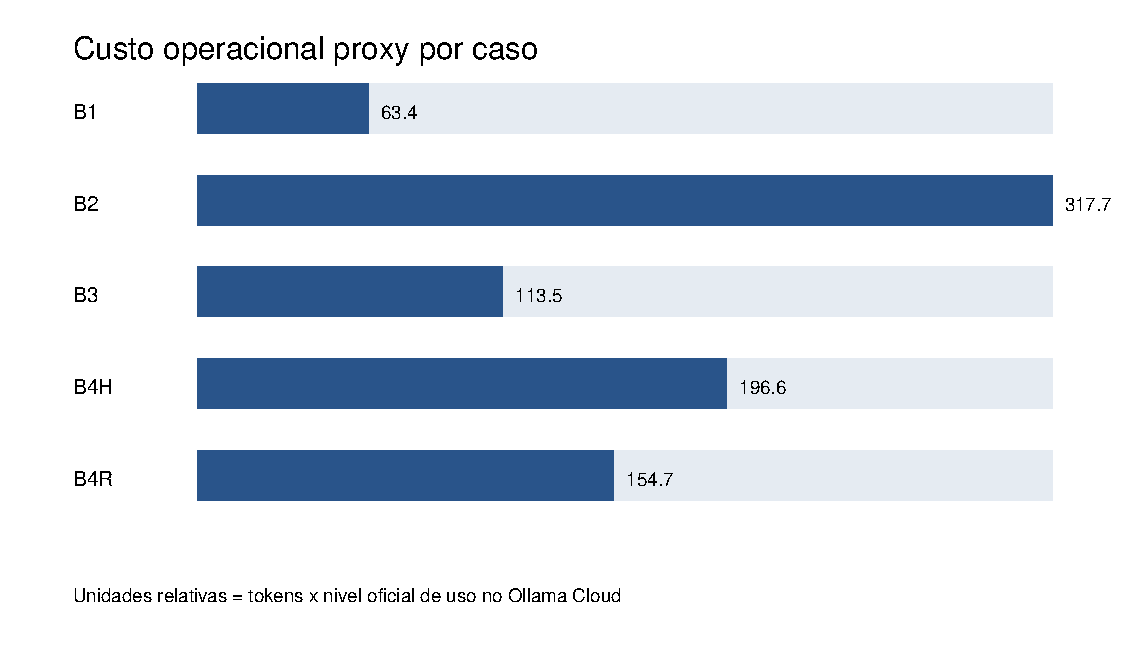
\includegraphics[width=.49\textwidth]{figures/cost_proxy.pdf}
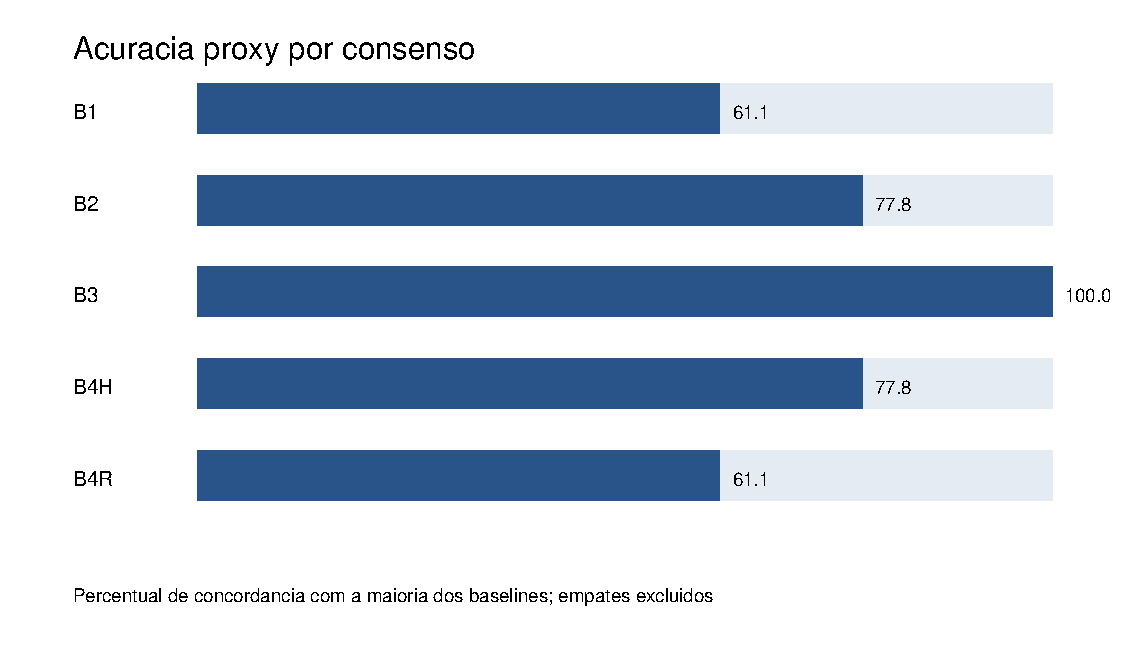
\includegraphics[width=.49\textwidth]{figures/accuracy_proxy.pdf}
\caption{Custo operacional proxy e acurácia proxy no subconjunto enriquecido. O custo proxy usa tokens multiplicados pelo nível oficial de uso do modelo no Ollama Cloud; a acurácia proxy mede concordância com o consenso dos baselines, não acerto financeiro real.}
\label{fig:custo-acuracia}
\end{figure*}

Os resultados mostram um trade-off mais claro do que a simples
distribuição de classificações. B1 é o modo mais barato e rápido, mas sua
concordância com o consenso é baixa. B2 melhora a concordância e produz a
maior quantidade média de fatores, porém é o modo mais caro em tokens e
uso proxy, pois executa cinco amostras sobre uma entrada enriquecida
longa. B3 aparece como o melhor ponto de equilíbrio nesta execução:
alcança 100\% de concordância com o consenso, mantém todos os diagnósticos
conclusivos e tem custo operacional menor que B2, B4-H e B4-R.

A comparação entre B4-H e B4-R é especialmente relevante para a proposta.
B4-R reduz o uso proxy em cerca de 21\% em relação a B4-H e também reduz
latência P95 e tentativas com erro. Isso sugere que o roteamento
heterogêneo é útil como mecanismo de controle de custo operacional. Ao
mesmo tempo, B4-R apresentou menor taxa de diagnósticos conclusivos e
menor concordância com o consenso. Assim, nesta rodada, a heterogeneidade
melhorou eficiência, mas não melhorou a proxy de acurácia.

\subsection{Discussão dos resultados}

Quatro pontos sustentam a leitura desses números. Primeiro, a arquitetura
é operacionalmente viável: todos os baselines executam sobre o mesmo
formato de entrada, produzem a mesma estrutura de saída e registram rastros
auditáveis. Segundo, a comparação financeira deve ser feita no cenário
enriquecido, porque ele fornece evidência de preço, fundamentos, notícias e
macroeconomia para todos os baselines. Terceiro, o debate adversarial ainda
não mostrou ganho claro de acurácia proxy sobre os baselines fortes. Nesta
execução, B3 superou B4-H e B4-R no trade-off entre consenso,
conclusividade e custo. Quarto, o roteamento heterogêneo de B4-R apresentou
ganho operacional em
relação a B4-H, mas esse ganho veio acompanhado de maior cautela e menor
concordância com o consenso.

Esses resultados deslocam a narrativa do artigo para uma conclusão mais
honesta. O trabalho não deve afirmar que debate multiagente é
automaticamente melhor. A evidência atual indica que a decomposição em
agentes ajuda a estruturar e auditar o diagnóstico financeiro, que B3 foi o
melhor modo de execução nesta rodada enriquecida e que o roteamento por
papel pode reduzir custo frente a uma versão homogênea. A validação de qualidade
econômica, erro factual detalhado e sensibilidade contrafactual por perfil
permanece necessária antes de afirmar superioridade financeira de B4.

\section{Ameaças à Validade}
\label{sec:ameacas}

Há ameaças importantes à validade dos resultados. As carteiras foram
obtidas de fontes públicas e podem não representar a distribuição
completa de carteiras reais de investidores; os perfis do workload,
além disso, não estão perfeitamente balanceados entre conservador,
moderado e agressivo. A validação estrutural não utiliza dados externos,
o que favorece diagnósticos inconclusivos nos sistemas que tratam
ausência de evidência com mais rigor, e deve ser lida como avaliação
estrutural, não como comparação principal de qualidade financeira.

A comparação enriquecida, por sua vez, foi feita em 20 carteiras. Ela é a
base da comparação entre técnicas, mas ainda é uma amostra limitada para
afirmar superioridade estatística de uma arquitetura sobre outra. Além
disso, parte dessa execução precisou ser realizada com menor concorrência
por instabilidade temporária do provedor, o que afeta diretamente as
métricas de latência. Os modelos usados via provedor externo podem variar
de comportamento ao longo do tempo, mesmo com prompts e entradas
congeladas. A métrica de acurácia proxy por consenso também pode favorecer
abordagens que se comportam de forma semelhante à maioria, sem garantir que
a maioria esteja correta financeiramente. E esta versão ainda não inclui
avaliação humana, LLM-as-judge calibrado, verificação detalhada de erro
factual nem comparação contra retorno futuro das carteiras.

Para reduzir esses riscos, o pipeline registra todas as chamadas e
resultados em SQLite, usa entradas congeladas, compara múltiplos
baselines, reporta erros de parsing e separa métricas operacionais de
métricas de qualidade. Mesmo assim, as conclusões aqui apresentadas
devem ser lidas como evidência inicial sobre a arquitetura e seu
comportamento, não como validação definitiva de desempenho financeiro.

\section{Conclusão}

Este trabalho apresenta uma arquitetura multiagente baseada em LLMs para
diagnóstico personalizado de carteiras financeiras. A proposta combina
agentes especializados, debate adversarial, moderação estruturada e
roteamento heterogêneo de modelos, mantendo a saída limitada a
diagnóstico e evitando recomendações de compra ou venda.

A contribuição central está na avaliação. O sistema é comparado contra
baselines fortes, incluindo agente único com self-consistency e
multiagente sem debate, e isso permite separar ganhos reais de
personalização e cobertura de risco de melhorias meramente textuais.
Os resultados mostram que a validação estrutural, sem dados externos,
expõe melhor como os sistemas multiagente tratam lacunas de evidência. A
comparação principal, feita com 20 carteiras enriquecidas, mostra diferenças
mais úteis entre os modos de execução: custo, latência, conclusividade,
detalhamento e concordância com consenso. Nesse cenário financeiro, B1 é o
mais barato, B2 é o mais detalhista em número de fatores, B3 apresenta o
melhor equilíbrio geral, e B4-R reduz custo e latência em relação a B4-H.

Assim, a principal conclusão não é que o debate adversarial já supera os
baselines em precisão financeira. Na execução enriquecida, B3 foi o melhor
equilíbrio entre concordância com consenso, diagnósticos conclusivos e custo
proxy, enquanto B4-R reduziu custo e latência em relação a B4-H, mas não
melhorou a proxy de acurácia. A conclusão mais defensável é que a
arquitetura proposta permite avaliar essa hipótese de forma controlada,
rastreável e comparável, e que o benefício do debate ainda precisa ser
demonstrado por métricas mais fortes. Como próximos passos, permanecem a
avaliação contrafactual por perfil, a verificação factual automática, a
calibração de LLM-as-judge com anotação humana e a comparação com desempenho
posterior das carteiras.



\begin{declarations}

\begin{acknowledgements}
Os autores agradecem à Universidade de Fortaleza (UNIFOR) pelo apoio institucional durante o desenvolvimento deste trabalho.
\end{acknowledgements}

\begin{funding}
Esta pesquisa não recebeu financiamento externo específico.
\end{funding}

\begin{contributions}
Rafael Florenzano contribuiu para a concepção do estudo, implementação dos agentes, mecanismo de debate, desenho experimental e redação principal do manuscrito. Rian Freitas contribuiu com infraestrutura, preparação de dados, execução experimental e revisão da metodologia. Ambos os autores leram e aprovaram o manuscrito final.
\end{contributions}

\begin{interests}
Os autores declaram que não têm nenhum conflito de interesses.
\end{interests}

\begin{materials}
Os conjuntos de dados e softwares gerados e/ou analisados durante o estudo atual serão disponibilizados em repositório público após a anonimização ou ao final do processo de revisão, conforme exigências do evento.
\end{materials}

\begin{furtherinformation}
Ferramentas de IA generativa foram utilizadas como apoio à redação técnica, sob revisão integral dos autores. Não houve necessidade de aprovação em comitê de ética, uma vez que o trabalho não envolve sujeitos humanos.
\end{furtherinformation}
\end{declarations}



\bibliographystyle{apalike-sol}
\bibliography{refs}

\end{document}
